\chapter{Classification: Alternative Techniques}

	\clearpage
	\section{Nearest-Neighbor Classifiers}

		Decision tree classifier are an example of {\bf eager learner} because
		they are designed to learn a model that maps the input attributes to 
		the class label as soon as the training data becomes available. 
		An opposite strategy would be to delay the process of modeling the 
		training data until it is needed to classify the test examples.
		Techniques that employ this strategy are known as {\bf lazy learners}.

		An obvious drawback of this approach is that some test records may not
		be classified because they do not match any training example. 
		One way to make this approach more flexible is to find all the
		training examples that are relatively similar to the attribues of the
		test example. These examples are known as {\bf nearest neighbors}.

		\vspace{0.3cm}
		{\it \Large "If it walks like a duck , quacks like a duck, and looks like a duck,
		then it's probably a duck."}

		\vspace{0.3cm}

		A nearest-neighbor classifier represents each example as a data point
		in a d-dimensional space, where d is the number of attributes. 
		The k-nearest neighbors of a given example {\it z} refer to the
		{\it k} points that are close to {\it z}.
		To classify an example it uses the {\bf majority} of classes closest to the point.

		In the picture below you can see K-nearest neighbors of a record x are data 
		points that have the k smallest distance to x. In the first picture, x will
		be classified as "negative" because the majority is "negative".
		In the second picture will be classified as "positve".
		In this situation when it is a {\bf tie}, we choose randomly. 
		In the last picture	we classify x as "positive" because the majoiry is "positive"
		
		\begin{figure}[H]
			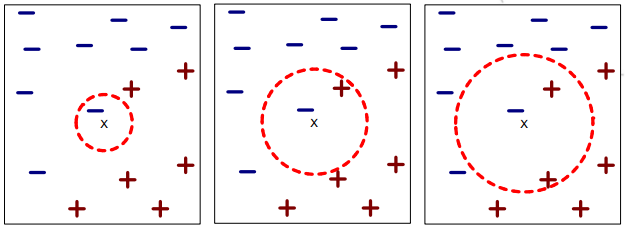
\includegraphics[width=\textwidth]{pics/knearest.png}
			\caption{1-nearest neighbor, 2-nearest neighbor and 3-nearest neighbor}
		\end{figure}

		You need to carefully pick the k because if its too small it can be close to noise
		so the classification is wrong. If the k is too big, it might happend that it
		will misclassify the test instance becuase its list of nearest neighbors may include
		data points that are located far away from its neighborhood.

		\clearpage
		\section{How to do the nearest-neighbor classifier}
		\clearpage
		{\bf The nearest-Neighbor Classifier algorithm needs:}
			\begin{itemize}
				\item The set of stored records 
				\item Distance Metric to compute 
				\item distance between records
				\item The value of k, the number of nearest neighbors to retrieve 
			\end{itemize}
		{\bf To classify an unknown record you need to:}
			\begin{itemize}
				\item Compute distance to other training records
				\item Identify k nearest neighbors 
				\item Use class labels of nearest neighbors to determine the class 
				label of unknown record (e.g., by taking majority vote)
			\end{itemize}

		{\bf Calculate the distance between two points usin the Euclidean distance:}
		\begin{equation}
			Euclidean distance = d(p,q) = \sum_{i}^{} \sqrt{(p_{i} - q_{i})^{2}}
		\end{equation}